\documentclass[border=10pt]{standalone}

\usepackage{tikz}
\usepackage{tikzsymbols}
\usetikzlibrary{calc,patterns,shapes.geometric}

\def\centerarc[#1](#2)(#3:#4:#5){\draw[#1] ($(#2)+({#5*cos(#3)},{#5*sin(#3)})$) arc (#3:#4:#5);}

\begin{document}
	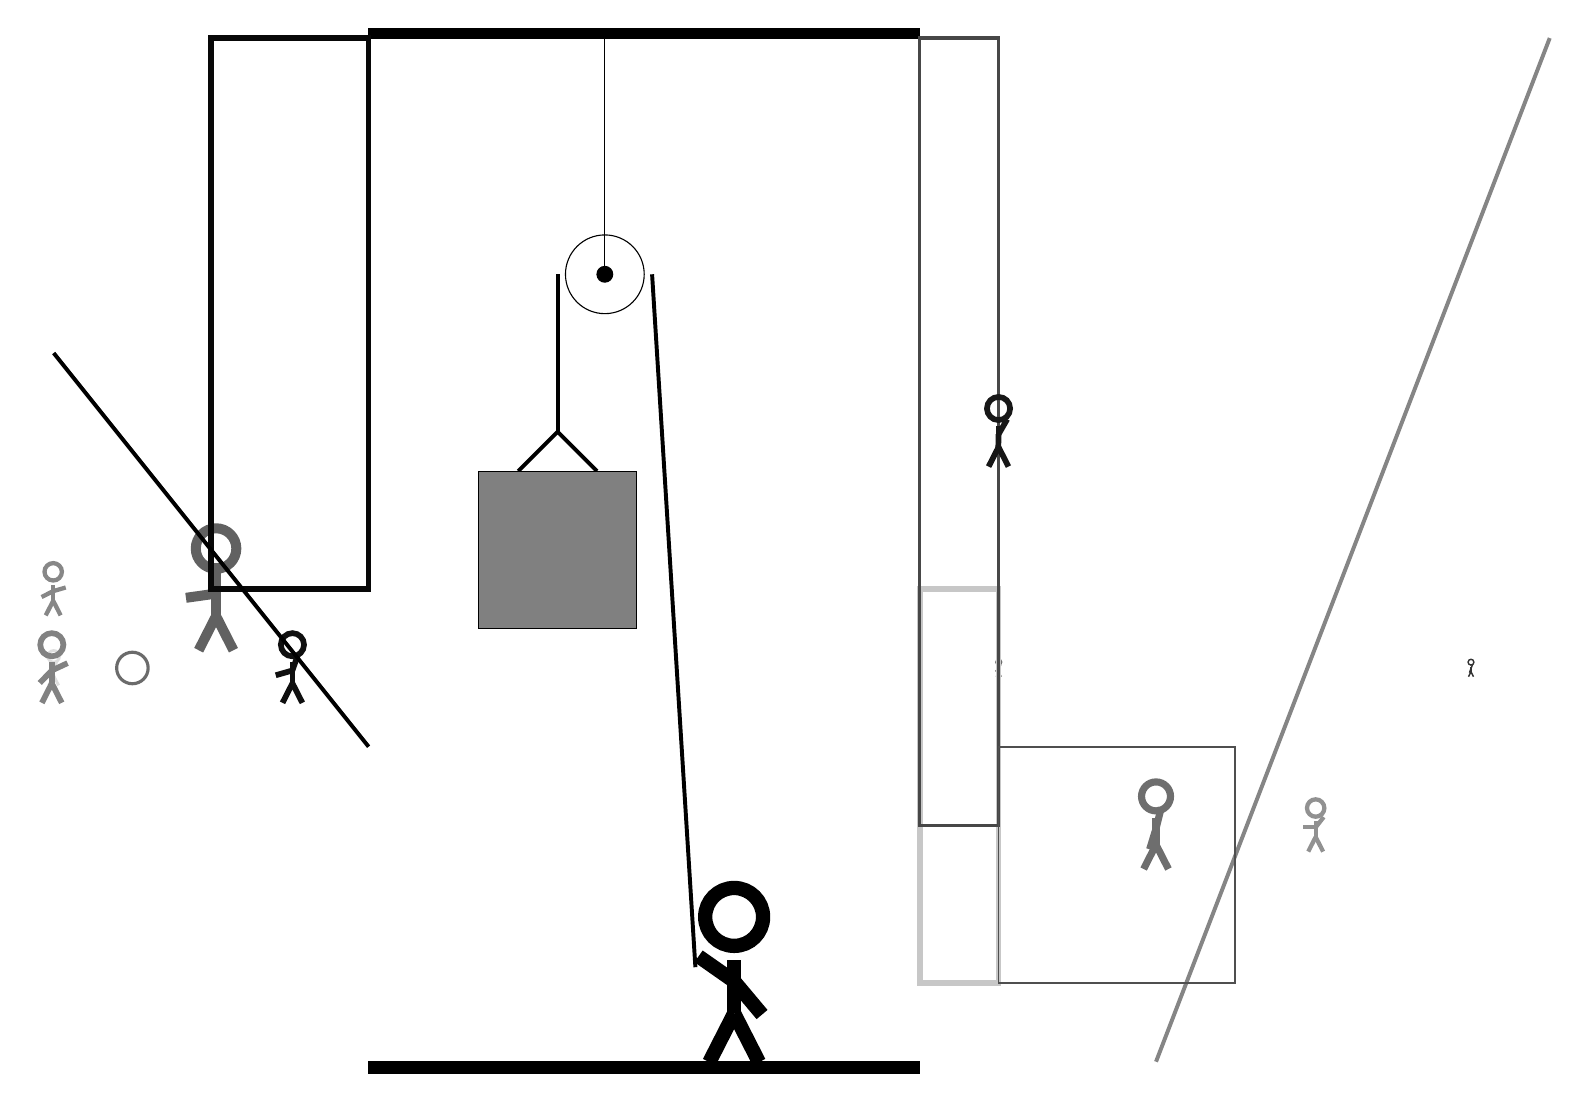
\begin{tikzpicture}
		%%%%% START %%%%%
		
		\draw[fill=black] (-2, 10) rectangle (5, 10.125);
		
		\draw (1, 7) circle (0.5);
		\draw[fill=black] (1, 7) circle (0.1);
		\draw (1, 10) -- (1, 7);
		
		\draw[line width=0.5mm] (-0.1, 4.5) -- (0.4, 5.0) -- (0.9, 4.5);
		\draw[fill=black!50] (-0.6, 4.5) rectangle (1.4, 2.5);
		
		\node[line width=0.3mm, color=black!13] at (-6, 2) {\Strichmaxerl[2][68][68]};
		
		\node[line width=0.6mm, color=black!80] at (12, 2) {\Strichmaxerl[1][69][69]};
		\node[line width=0.2mm, color=black!49] at (-6, 2) {\Strichmaxerl[4][46][25]};
		\node[line width=0.2mm, color=black!57] at (6, 2) {\Strichmaxerl[1][40][61]};
		
		\draw [line width=0.4mm, color=black!58](-5, 2) circle (0.2);
		
		\draw[line width=0.7mm, color=black!22] (6, -2) rectangle (5, 3);
		
		\draw[line width=0.5mm, color=black!48](8, -3) -- (13, 10);
		\node[line width=0.6mm, color=black!94] at (-3, 2) {\Strichmaxerl[4][16][71]};
		\node[line width=0.6mm, color=black!47] at (-6, 3) {\Strichmaxerl[3][27][16]};
		\node[line width=0.6mm, color=black!62] at (-4, 3) {\Strichmaxerl[7][8][90]};
		
		\draw[line width=0.4mm, color=black!72] (5, 10) rectangle (6, 0);
		\node[line width=0.2mm, color=black!57] at (8, 0) {\Strichmaxerl[5][73][76]};
		\draw[line width=0.7mm, color=black!97] (-2, 3) rectangle (-4, 10);
		
		\draw[line width=0.2mm, color=black!69] (6, 1) rectangle (9, -2);
		\node[line width=0.3mm, color=black!43] at (10, 0) {\Strichmaxerl[3][0][52]};
		\node[line width=0.2mm, color=black!91] at (6, 5) {\Strichmaxerl[4][89][60]};
		
		\draw[line width=0.5mm, color=black!100](-6, 6) -- (-2, 1);
		
		
		\draw[line width=0.5mm] (0.4, 7) -- (0.4, 5.0);
		\centerarc[line width=0.5mm](1, 7)(0:180:0.6);
		\draw[line width=0.5mm](1.6, 7) -- (2.15, -1.8);
		
		\node at (2.6, -1.9) {\Strichmaxerl[10][-35][-50]};
		
		\draw[fill=black] (-2, -3) rectangle (5, -3.15);
		
		%%%%% END %%%%%
	\end{tikzpicture}
\end{document}